\documentclass[11pt]{article}\usepackage[]{graphicx}\usepackage[]{color}
% maxwidth is the original width if it is less than linewidth
% otherwise use linewidth (to make sure the graphics do not exceed the margin)
\makeatletter
\def\maxwidth{ %
  \ifdim\Gin@nat@width>\linewidth
    \linewidth
  \else
    \Gin@nat@width
  \fi
}
\makeatother

\definecolor{fgcolor}{rgb}{0.345, 0.345, 0.345}
\newcommand{\hlnum}[1]{\textcolor[rgb]{0.686,0.059,0.569}{#1}}%
\newcommand{\hlstr}[1]{\textcolor[rgb]{0.192,0.494,0.8}{#1}}%
\newcommand{\hlcom}[1]{\textcolor[rgb]{0.678,0.584,0.686}{\textit{#1}}}%
\newcommand{\hlopt}[1]{\textcolor[rgb]{0,0,0}{#1}}%
\newcommand{\hlstd}[1]{\textcolor[rgb]{0.345,0.345,0.345}{#1}}%
\newcommand{\hlkwa}[1]{\textcolor[rgb]{0.161,0.373,0.58}{\textbf{#1}}}%
\newcommand{\hlkwb}[1]{\textcolor[rgb]{0.69,0.353,0.396}{#1}}%
\newcommand{\hlkwc}[1]{\textcolor[rgb]{0.333,0.667,0.333}{#1}}%
\newcommand{\hlkwd}[1]{\textcolor[rgb]{0.737,0.353,0.396}{\textbf{#1}}}%
\let\hlipl\hlkwb

\usepackage{framed}
\makeatletter
\newenvironment{kframe}{%
 \def\at@end@of@kframe{}%
 \ifinner\ifhmode%
  \def\at@end@of@kframe{\end{minipage}}%
  \begin{minipage}{\columnwidth}%
 \fi\fi%
 \def\FrameCommand##1{\hskip\@totalleftmargin \hskip-\fboxsep
 \colorbox{shadecolor}{##1}\hskip-\fboxsep
     % There is no \\@totalrightmargin, so:
     \hskip-\linewidth \hskip-\@totalleftmargin \hskip\columnwidth}%
 \MakeFramed {\advance\hsize-\width
   \@totalleftmargin\z@ \linewidth\hsize
   \@setminipage}}%
 {\par\unskip\endMakeFramed%
 \at@end@of@kframe}
\makeatother

\definecolor{shadecolor}{rgb}{.97, .97, .97}
\definecolor{messagecolor}{rgb}{0, 0, 0}
\definecolor{warningcolor}{rgb}{1, 0, 1}
\definecolor{errorcolor}{rgb}{1, 0, 0}
\newenvironment{knitrout}{}{} % an empty environment to be redefined in TeX

\usepackage{alltt}
%\usepackage[showframe]{geometry}
\usepackage[table]{xcolor}
\usepackage{caption}
\usepackage{lscape,verbatim,mathrsfs}
\usepackage{graphics,amsmath,pstricks}
\usepackage{amssymb,enumerate}
\usepackage{amsbsy,amsmath,amsthm,amsfonts, amssymb}
\usepackage{graphicx, rotate, array}
\usepackage{geometry,multirow}
\usepackage{color,soul}
\usepackage{float}
%\usepackage{hyperref}
\usepackage[authoryear,round]{natbib}
%\renewcommand{\baselinestretch}{1.9}
\usepackage{tcolorbox}
\renewcommand{\familydefault}{cmss}
\textwidth=6.65in \textheight=9.7in
\parskip=.025in
\parindent=0in
\oddsidemargin=-0.1in \evensidemargin=-.1in \headheight=-.6in
\footskip=0.5in \DeclareMathOperator*{\argmax}{argmax}
\DeclareMathOperator*{\argmin}{argmin}
\IfFileExists{upquote.sty}{\usepackage{upquote}}{}
\begin{document}











\section{Description of DGP}

\begin{align*}
W_1,W_2,W_3,W_4 &\sim Normal(\mu=0,\sigma^2=1) \\
A &\sim Bernoulli(p=0.5) \\
Y &\sim Bernoulli(p) \text{ .}\\
\end{align*}
\begin{align*}
p &= 0.5*logit^{-1} (1-W_1^2  + 3W_2  + 5W_3^2 A - 4.45A)+0.5logit^{-1} (-0.5- W_3  + 2W_1 W_2  + 3|W2|A - 1.5A) \text{ ,}
\end{align*}
True blip function is:
\begin{align*}
B_0 (W)= & 0.5[logit^{-1} (1-W_1^2  + 3W_2  + 5W_3^2  - 4.45)+logit^{-1} (-0.5- W_3  + 2W_1 W_2  + 3|W2|  - 1.5)\\
& - logit^{-1} (1-W_1^2  + 3W_2 )+logit^{-1} (-0.5- W_3  + 2W_1 W_2 )] \text{ .}
\end{align*}


\section{Library legend}

\begin{itemize}
\item Simple - GLMs
\begin{itemize}
\item QAW.SL.library = linear model with $W_j$ and A as main terms and $W_j$*A interaction for each $j$
\item blip.SL.library = linear model with main terms $W_j$ for each $j$
\end{itemize}
\item Medium - ML + GLMs not aggressive
\begin{itemize}
\item QAW.SL.library = GLMs library AND SL.glm, SL.mean, SL.glm.interaction, SL.earth, SL.nnet, SL.svm, SL.rpart
\item blip.SL.library = GLMs library AND SL.glm, SL.mean, SL.glm.interaction, SL.earth, SL.nnet, SL.svm, SL.rpart
\end{itemize}
\item Aggressive - ML + GLMs not aggressive
\begin{itemize}
\item QAW.SL.library = ML + GLMs aggressive library AND SL.randomForest
\item blip.SL.library = ML + GLMs aggressive library AND SL.randomForest
\end{itemize}
\end{itemize}






\subsection{Table Simple Library}
\begin{knitrout}
\definecolor{shadecolor}{rgb}{0.969, 0.969, 0.969}\color{fgcolor}\begin{kframe}
\begin{verbatim}
## $table_EnYdn_for_E0Yd0
##                Bias Variance    MSE Coverage
## Psi_gcomp   -0.0765    3e-04 0.0062        -
## Psi_IPTW    -0.0569    8e-04 0.0041    45.7%
## Psi_IPTW_DR -0.0565    7e-04 0.0038    29.8%
## Psi_TMLE    -0.0563    7e-04 0.0038    29.4%
## Psi_CV.TMLE -0.0752    9e-04 0.0066      14%
## 
## $table_EnYd0_for_E0Yd0
##                Bias Variance   MSE Coverage
## Psi_gcomp   -0.0935    2e-04 9e-03        -
## Psi_IPTW    -0.0004    8e-04 8e-04    95.8%
## Psi_IPTW_DR  0.0002    4e-04 4e-04    95.8%
## Psi_TMLE     0.0004    4e-04 4e-04    95.8%
## Psi_CV.TMLE  0.0007    5e-04 5e-04    95.3%
## 
## $table_EnYdn_for_E0Ydn
##                Bias Variance    MSE Coverage
## Psi_gcomp   -0.0035    3e-04 0.0004        -
## Psi_IPTW     0.0162    8e-04 0.0011    94.9%
## Psi_IPTW_DR  0.0166    7e-04 0.0009    90.6%
## Psi_TMLE     0.0167    7e-04 0.0009    90.5%
## Psi_CV.TMLE  0.0002    9e-04 0.0009    93.9%
\end{verbatim}
\end{kframe}
\end{knitrout}
\subsection{Table Medium Library}
\begin{knitrout}
\definecolor{shadecolor}{rgb}{0.969, 0.969, 0.969}\color{fgcolor}\begin{kframe}
\begin{verbatim}
## $table_EnYdn_for_E0Yd0
##                Bias Variance    MSE Coverage
## Psi_gcomp   -0.1248   0.0005 0.0161        -
## Psi_IPTW     0.0341   0.0011 0.0022    75.7%
## Psi_IPTW_DR  0.0352   0.0009 0.0021    64.2%
## Psi_TMLE     0.0331   0.0008 0.0019    64.5%
## Psi_CV.TMLE -0.0297   0.0008 0.0016    71.4%
## 
## $table_EnYd0_for_E0Yd0
##                Bias Variance    MSE Coverage
## Psi_gcomp   -0.1235    5e-04 0.0157        -
## Psi_IPTW    -0.0011    8e-04 0.0008    95.2%
## Psi_IPTW_DR -0.0011    5e-04 0.0005    94.8%
## Psi_TMLE    -0.0009    5e-04 0.0005    94.9%
## Psi_CV.TMLE -0.0008    5e-04 0.0005    95.4%
## 
## $table_EnYdn_for_E0Ydn
##                Bias Variance    MSE Coverage
## Psi_gcomp   -0.0977   0.0005 0.0101        -
## Psi_IPTW     0.0612   0.0011 0.0048    45.3%
## Psi_IPTW_DR  0.0623   0.0009 0.0048    29.1%
## Psi_TMLE     0.0602   0.0008 0.0044      30%
## Psi_CV.TMLE  0.0002   0.0008 0.0008    94.3%
\end{verbatim}
\end{kframe}
\end{knitrout}
\subsection{Table Aggressive Library}
\begin{knitrout}
\definecolor{shadecolor}{rgb}{0.969, 0.969, 0.969}\color{fgcolor}\begin{kframe}
\begin{verbatim}
## $table_EnYdn_for_E0Yd0
##                Bias Variance    MSE Coverage
## Psi_gcomp   -0.1165   0.0006 0.0142        -
## Psi_IPTW     0.1076   0.0104 0.0220    40.5%
## Psi_IPTW_DR  0.0995   0.0102 0.0201    36.6%
## Psi_TMLE     0.1004   0.0115 0.0216    36.9%
## Psi_CV.TMLE -0.0278   0.0007 0.0014    74.8%
## 
## $table_EnYd0_for_E0Yd0
##                Bias Variance    MSE Coverage
## Psi_gcomp   -0.1170    6e-04 0.0142        -
## Psi_IPTW     0.0020    8e-04 0.0008    95.8%
## Psi_IPTW_DR -0.0036    5e-04 0.0005    93.9%
## Psi_TMLE    -0.0034    5e-04 0.0005    94.4%
## Psi_CV.TMLE  0.0011    5e-04 0.0005    95.7%
## 
## $table_EnYdn_for_E0Ydn
##                Bias Variance    MSE Coverage
## Psi_gcomp   -0.0868   0.0006 0.0081        -
## Psi_IPTW     0.1373   0.0104 0.0292    25.4%
## Psi_IPTW_DR  0.1292   0.0102 0.0269    20.5%
## Psi_TMLE     0.1301   0.0115 0.0285      20%
## Psi_CV.TMLE  0.0003   0.0007 0.0007      95%
\end{verbatim}
\end{kframe}
\end{knitrout}



\section{Results}
\begin{knitrout}
\definecolor{shadecolor}{rgb}{0.969, 0.969, 0.969}\color{fgcolor}
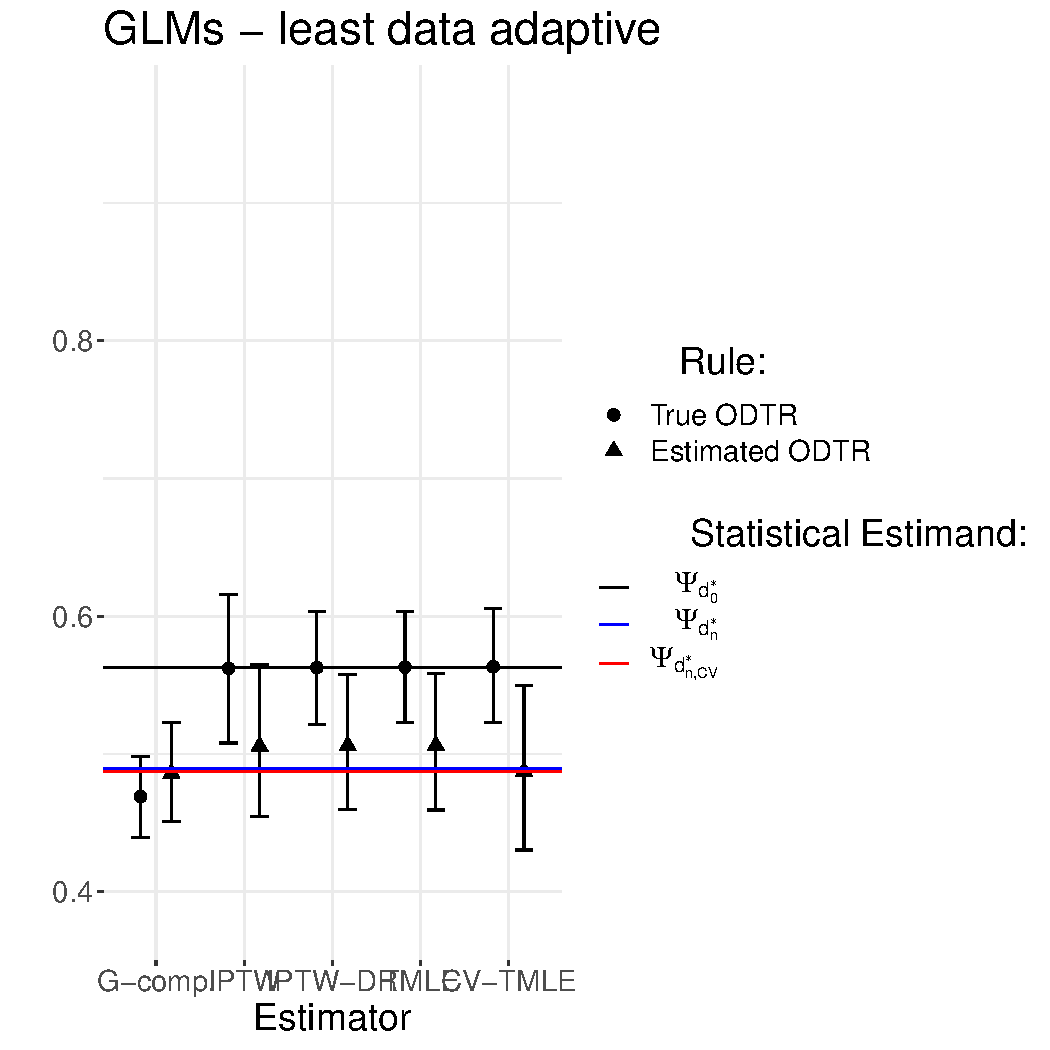
\includegraphics[width=\maxwidth]{figure/unnamed-chunk-6-1} 

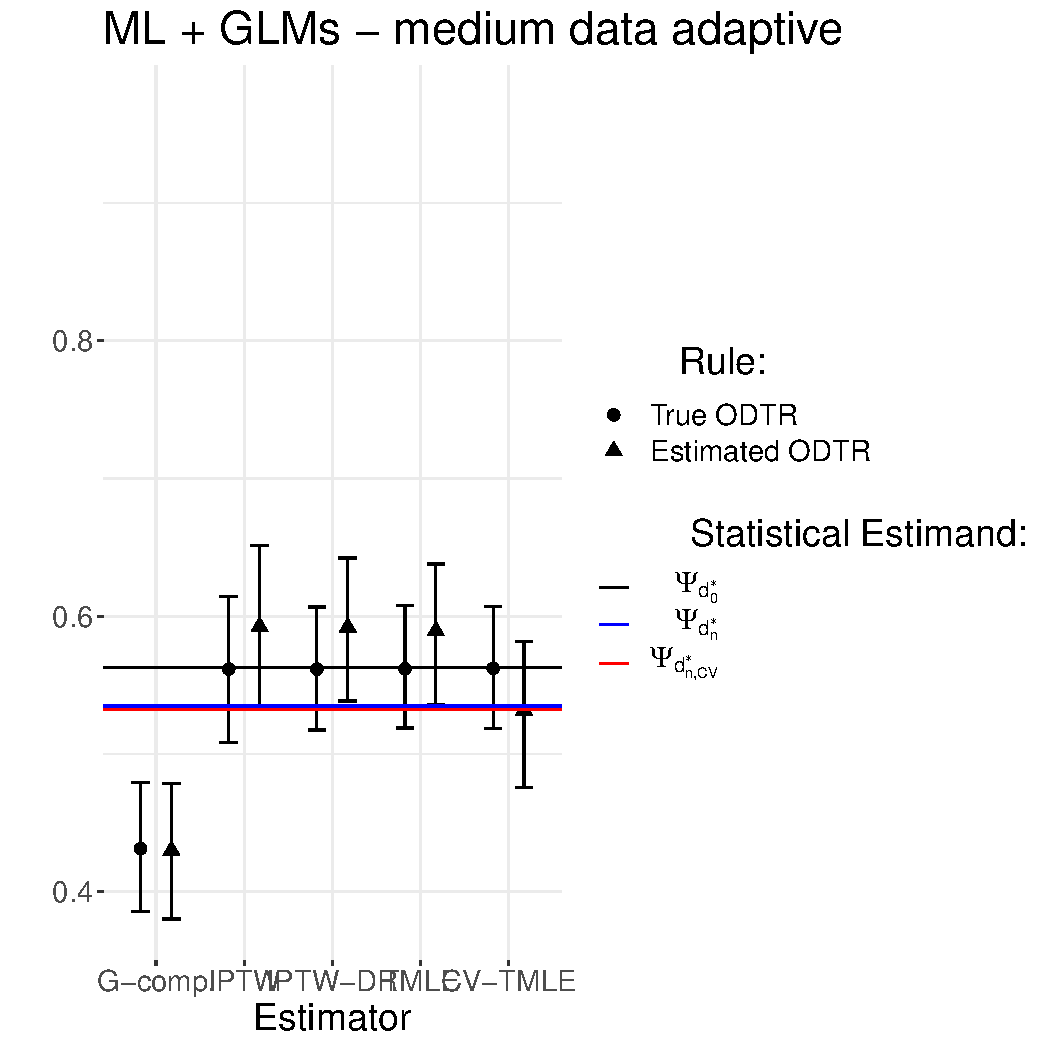
\includegraphics[width=\maxwidth]{figure/unnamed-chunk-6-2} 

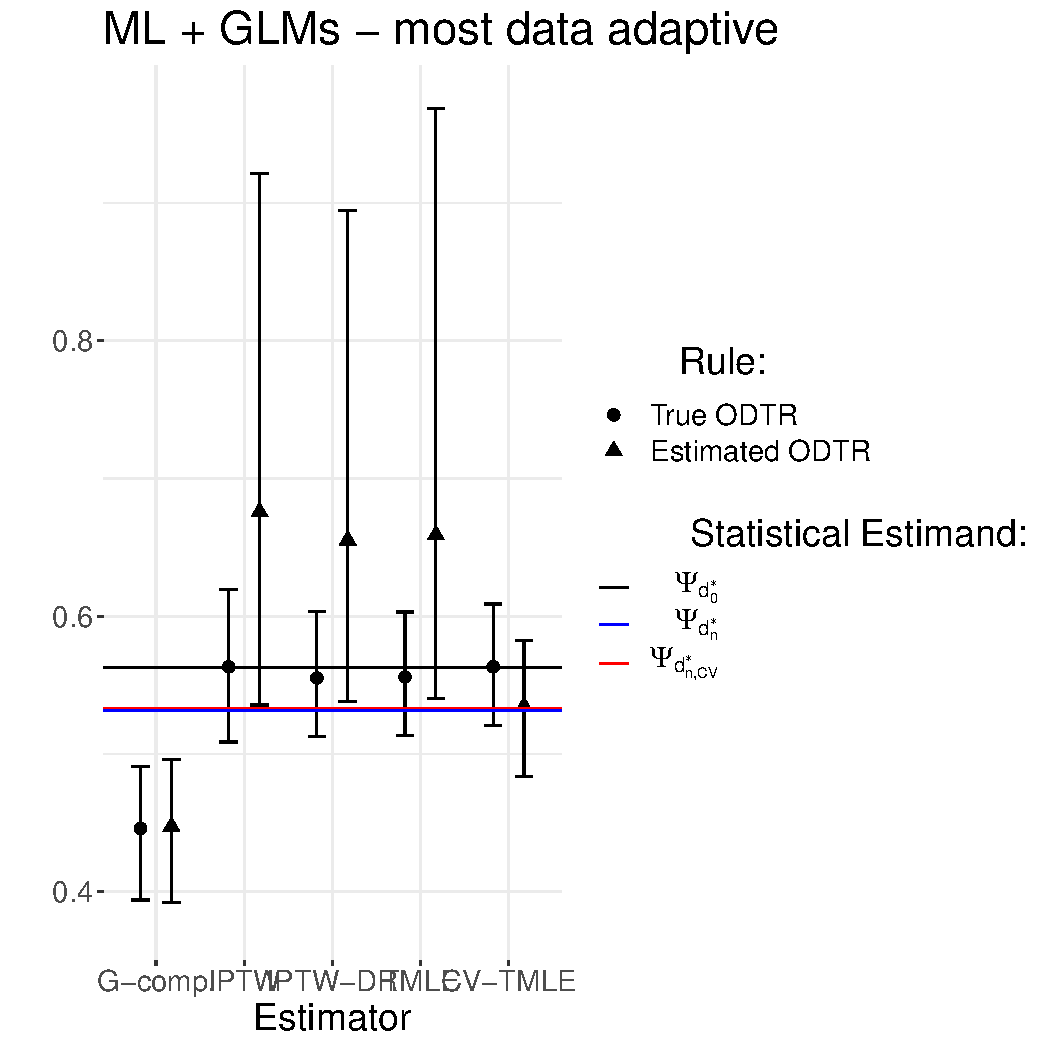
\includegraphics[width=\maxwidth]{figure/unnamed-chunk-6-3} 

\end{knitrout}

\end{document}
